% !TEX root = ../../../../main/numb3rs_activities.tex
\newpage
\phantomsection
\addcontentsline{toc}{subsection}{204: Calculated Risk \label{ep204}}
\ep{204: Calculated Risk}
\setcounter{activity}{0}

In the episode Calculated Risk, Charlie is trying to track the movement of money through a company in order to figure out who is profiting from a series of illegal trades. While discussing the problem in his office, Professor Fleinhardt in distracted by a pool of standing water in the corner. To find the source of the leak, Fleinhardt spreads ink in the water to observe the flow. Quite to the opposite of expectation, he sees that the water is not dripping down from the ceiling, but in fact rising up from the floor. Thinking that the movement of funds in a company is not entirely unlike a flow, Charlie realizes that the money must have been diverted before the illegal trades even took place. \\


% Flows
\ltLarge{Flows}


Flows can help scientists understand a number of phenomena, particularly the movement of liquids and gases. To a mathematician, a flow is a specific kind of function designed to describe such behavior. Recall that we can think of functions as ``black boxes'' that, given input, output a number. A function is \emph{well-defined} as long as its output is uniquely determined by the input. Although you may be accustomed to dealing with functions of one variable such as $f(x) = 3x + 2$, $f(x)= \sin x$, etc, there is no reason why functions cannot have more complicated inputs. The input for a flow is given by a pair $(p,t)$, where $p$ represents a point in space (the initial placement of a particle) and $t$ represents the amount of time that has elapsed since the particle was released in the flow. The function returns the current position of the particle.


To see a flow for yourself, simply turn on the weather channel and watch the movement of clouds. If you had a long enough movie, you could fast forward, rewind, and pause to see where the wind would be taking, say, a tiny bit of pollen. Note that we are concerned with the movement of the air itself, not with the formation and dispersion of individual clouds. Like the ink used by Fleinhardt, the clouds just make the flow easier to see. Since flows are designed to model physical behavior, they have additional restrictions. Flows must be continuous, meaning there are no sudden jumps or changes in the movement of a particle. After all, we can't have our pollen teleporting about! There is one additional restriction on a function of two variables that makes it a flow, see if you can figure this restriction out for yourself by filling in the blank:
	\[
	f(f(p,t_1),t_2)= f(p,\underline{\phantom{xxxxx}}\;)
	\]
Use a picture to convince yourself why this restriction should always be satisfied by a function called a ``flow.''


One problem with flows is that they are difficult to draw. With functions of one variable, only two dimensions are needed for a graph: one for the input and one for the output. If we were trying to represent the behavior of a flow in 3 dimensional space, how many dimensions would we need to hold all of the information? \\
	\begin{figure}[H]
	\centering
	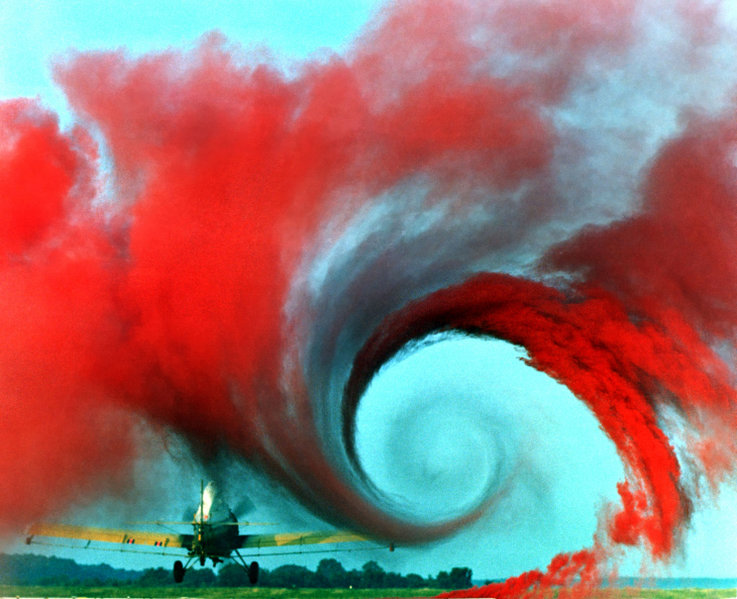
\includegraphics[width=0.5\textwidth]{season2/204/images/vortexflow.jpg} 
	\end{figure}
A representation of a flow can be given by drawing flow lines on a space. Each flow line is determined by fixing an initial position and letting $t$ vary. So, every particle that starts on a given flow line will always stay on that line. Note: although we do not often think of time as being negative, it is convenient to be able to determine where a particle has been, as well as where it is going. Therefore, $\phi(p,-5)$, outputs where a particle in position p must have been 5 seconds ago. Here is an example of a flow represented by flow lines:
	\begin{figure}[H]
	   \centering
	   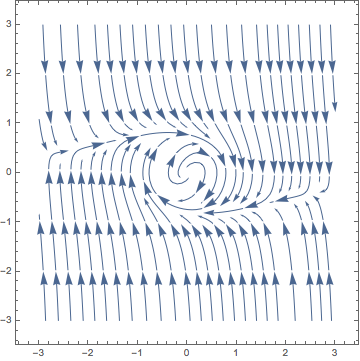
\includegraphics[width=0.4\textwidth]{season2/204/images/flow.png} 
	\end{figure}
Flows can be restricted to all kinds of interesting spaces. Here, we discuss flows on a few familiar surfaces. Recall, the domain of the flow includes the entire space and a time dimension, while the range of the flow is the space itself. \\

	\begin{itemize}
	\item Describe a nowhere stationary flow on the unit circle by precisely describing the motion of a particle.
	\item The outer skin of a donut forms a space known as the torus. Describe a nowhere stationary flow on the torus. Draw a torus with the appropriate flow lines. Hint: Use your answer above.
	\begin{figure}[H]
	   \centering
	   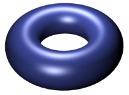
\includegraphics[width=0.3\textwidth]{season2/204/images/bluetorus.png} 
	\end{figure}
	\item It is a deep theorem of mathematics that you cannot construct a nowhere stationary flow on the surface of a sphere. Try constructing such a flow, and see what happens. Why do you think this theorem is often referred to as ``You Can't Comb a Coconut''?
	\end{itemize}

